\chapter{Introduction}

Dust is a flexible solution to simulate the aerodynamics of complex, non-conventional aircraft configuration.

It consists of three executables which are meant to perform preprocessing of the geometry, run the simulation in the desired condition and then postprocess the results obtained to gather the required meaningful data. 

\section{Workflow}
\label{sec:Workflow}

The most typical workflow with DUST is illustrated in figure \ref{fig:worflow}.  The geometry of the solid bodies, in form of cgns mesh or parametric directive, must be provided to the preprocessor, which performs preliminary operations and generates a binary geometry file. 

Such file is provided, alongside the parameters for the simulation and the reference frames, to the solver, which executes the simulation and produces the complete results inside binary files. 

The produced results contain the complete solution obtained during the simulation, in terms of distribution of singularities on body surfaces and wake. However it is difficult to obtain condensed, meaningful data from such results.

For this reason it is possible to specify a variety of different analyses to be performed by the postprocessor, which employs the global results to generate a series of different meaningful results, from visualization and flow fields to loads and loads distribution, in different formats.

\begin{figure}[h]
\centering
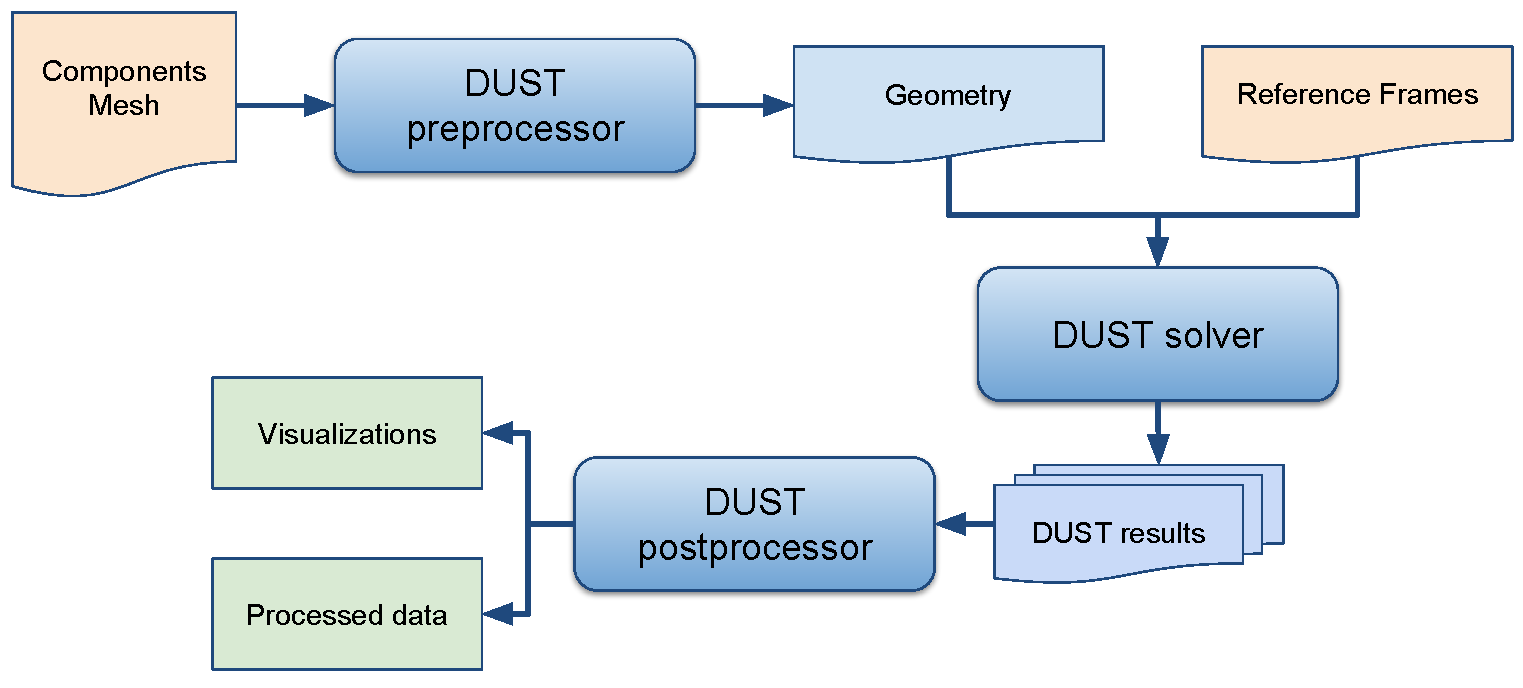
\includegraphics[width=\textwidth]{Workflow}
\caption{Description of the worflow with DUST}
\label{fig:worflow}
\end{figure}



\section{Input Files Format}
\label{sec:InputFilesFormat}
All the input files, which are used to define parameters to the DUST executables, share the same flexible, free format text files structure.

The files are simple text files, without any requirement on the extension, however the extension \texttt{*.in} is recommended to distinguish the input files inside the case folders. The different executables automatically look for the input file \texttt{exe\_name.in} where they are invoked. 

An example of text input file is presented in file \ref{file:example}. Input files employ loosely a Fortran syntax, and comprise of a series of keyword assignments.
The required keyword can generally be inserted in any order inside the input file, and should be written according to the following rules:
\begin{itemize}
\item All the parameters assignments are written with an equal sign, i.e. keyword = value, for any kind of value.
\item Extra spaces and blank lines are ignored
\item Comments are introduced with an exclamation mark "!", and can be introduced at the beginning of a line, or after a valid keyword assignment.
\item Strings are introduced \emph{as they are}, without quotes, and will be automatically stripped of leading and trailing spaces
\item Integer and real numbers are introduced as usual, also with exponential notation
\item Logicals are introduced as "T" for true and "F" for false
\item Arrays can be introduced with the Fortran notation: contained between brackets and slashes and with elements separated by comas. 
\item Some keywords might be required to be contained inside a grouping keyword. It is a keyword which contains another set of keywords inside curly brackets. 
\end{itemize}

\begin{inputfile}[frame=single, caption={example input file}, label={file:example}]
! comments are introduced with an exclamation mark as in Fortran
ExampleString   = a_string
ExampleInteger  = 59
ExampleReal     = 67.84 !all comments even inline are ignored
ExampleLogical  = T     !as well as all the extra spaces.

!empty lines are ignored
ExampleArray = (/ 0.5, 2.3e-3, 5.67329/)

ExampleMultiple = 1.3
ExampleMultiple = 7.2 !some keywords can have multiple values

!some keyword can require to be grouped inside another grouping keyword
ExampleGrouping = {
	GroupedVarInt = 5 !indenting can be helpful, but is not required
    GroupedVarLogical = F
}
\end{inputfile}

Regarding the number, position and compulsoriness of the keywords, depending on the keyword:
\begin{itemize}
\item Some keyword can be required and compulsory, some can be optional, in the sense that a default value is employed if the keyword is not defined, and also can be required only in specific cases, according choices made in other parameters (e.g. if the user requires a simulation to be restarted from file, should provide the file name, otherwise the file name keyword can be neglected)
\item Some keyword can be multiple: if the user should provide a list of a series of entities a keyword can be repeated several times
\item Some keyword, contrary to all the other, must be placed in precise relative position (before/after) another keyword, due to the strong correlation of the parameters.
\end{itemize}
All the details on the parameters of the single files will be provided in the description of each input file in the following chapters.

\section{Internal Binary Files Format}
\label{sec:BynaryFilesFormat}
All the files that contain data, input geometry and results, which are not meant to be interpreted by the user but are only for internal use, are written in binary hdf5 format. 

The hdf5 format is a common opensource binary format which allows to store efficiently both in terms of size and I/O speed a variety of data in a single file. 

The standard extension for hdf5 files is \texttt{.h5} and, even if it is not compulsory, should be added to the binary filenames in the parameter when specified.

\section{Output Files Format}
\label{sec:OutputFilesFormat}

As previously discussed in section \ref{sec:Workflow} the binary files results are not meant to be interpreted by the user (even if the use of applications as hdfView can give a brief insight on some results). The postprocessor can interpret those results and output processed data readily employable by the user.

Most of the postprocessed results can be obtained in Tecplot binary (\texttt{}) format, which is compact and convenient. However Tecplot is a proprietary software available only under licence. For this reason all the results can also be produced in the standard vtk format for visualizations (that can be opened by a variety of programs, e.g. paraview or visit) and formatted ascii files for line plots. 

Ascii files are also employed for analyses which output a single set of values (which are not meant to be plotted) and are convenient to be read inside automated execution loops. 